% \chapter{Fungsi (Subprogram)}
% \section{Tujuan}
\section{Goals}
\begin{itemize}[label=$\bullet$, itemsep=-1pt, leftmargin=*]
    \item Students are able to create and call functions in C .
          % \item Mahasiswa mengerti cara membuat dan memanggil fungsi pada bahasa pemrograman C.
    \item Students are able to pass parameter by value and by reference in C.
          % \item Mahasiswa mampu menggunakan passing parameter by value dan by reference pada bahasa pemrograman C.
    \item Students understand and are able to apply recursion in C.
          % \item Mahasiswa mampu mengerti dan mengaplikasikan konsep rekursi pada bahasa pemrograman C.

\end{itemize}

% \section{Fungsi}
\section{Function}
% Fungsi adalah sebuah kumpulan statement untuk melakukan tugas spesifik, yang bisa membutuhkan input ataupun tidak, untuk menghasilkan output yang sesuai.
A function is a collection of statment that is used to perform a spesific task, it may or may not use an input to generate the desired output.
These are the advantages of using functions in C programming language are:
% Keuntungan menggunakan fungsi pada bahasa pemrograman C adalah:
\begin{itemize}
    \item Some code snippets are reusable when using functions.
          % \item Beberapa cuplikan kode dapat digunakan kembali saat menggunakan fungsi.
    \item C functions can be called any number of times in a program and at any place in a program.
          % Kita dapat memanggil fungsi C berapa kali pun dalam suatu program dan dari mana saja dalam suatu program.
    \item A complex and large C codes can be splitted to several function, thus easier to track.
          % \item Program c yang besar dapat dibagi ke dalam beberapa fungsi sehingga dapat dengan mudah untuk dilacak.
\end{itemize}
\subsection{Function Declaration}
Every C program has atleast one function, which is the main() function. You can also define functions other than main().
% Setiap program C mempunyai minimal satu fungsi, yaitu fungsi main(). Anda juga dapat mendefinisikan fungsi selain main()
Syntax :
\begin{verbatim}
    return_type function_name( parameters list){
        // function body
    	return something;
    }
\end{verbatim}
\begin{itemize}
    \item Return Type.\\ The data type a function has to return.
          % \item Return Type.\\ Tipe data yang harus dikembalikan suatu fungsi.
    \item \verb*|function_name|.\\ The name of the function
          % \item \verb*|function_name|.\\ Nama fungsi
          % \item parameters list.\\  
    \item parameters list.\\
          % Parameter dari fungsi.
          The parameters of the function.
    \item Function body.\\ The block of code (Statements) that will be executed when the function is called.
          % \item Function body.\\ Kumpulan statemen yang mendefinisikan apa yang dilakukan oleh fungsi.
    \item \verb|return something;|\\ A statement to return a value (\verb|something|) from the function \verb*|function_name|.
          Returning causes the program to break out of the function.
          For functions that doesn't return a value (\verb|void| type function), to break out of a function simply write \verb|return;|
          % \item \verb|return something;|\\ merupakan statement untuk mengembalikan nilai dari fungsi. 
          % Untuk fungsi yang tidak mengembalikan nilai, dapat digunakan \verb|return_type| \verb|void|. 
          % Untuk keluar dari fungsi itu hanya perlu menggunakan statement \verb*|return|
\end{itemize}

Example
% Contoh

\begin{lstlisting}[language=c]
float TriangleArea(float Base, float Height)
{
	float Area;
	Area = 0.5*Base*Height;
	return Area;
}
\end{lstlisting}


\subsection{Calling a Function}
% \subsection{Memanggil Fungsi} 

\begin{figure}[H]
    \centering
    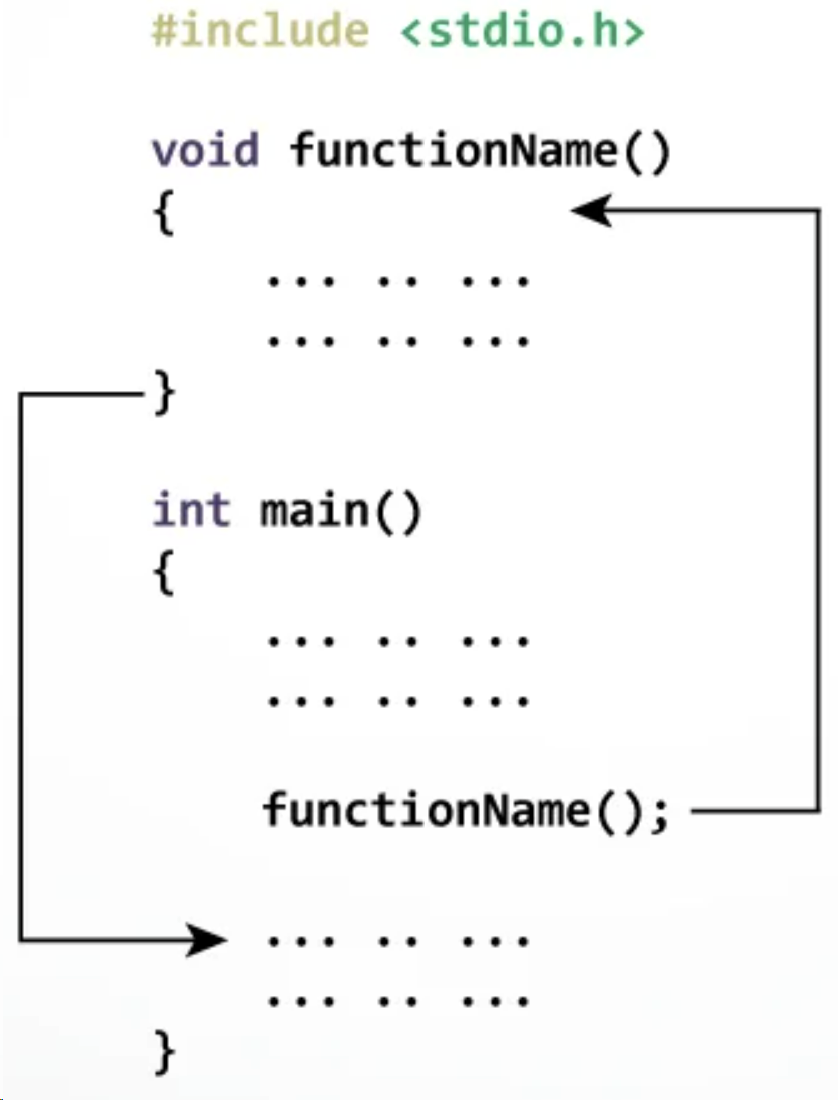
\includegraphics[width=0.45\linewidth]{P3/img/screenshot005.png}
    \caption{}
    \label{fig:memanggilfungsi}
\end{figure}

\begin{lstlisting}[language=c]
	#include <stdio.h>
  // Declaring a function to calculate a Triangle Area called TriangleArea  
% // Mendeklarasikan fungsi luasSegitiga
  // The parameters are the  value of Base and Height
% // Parameter input Alas , dan Tinggi
  // The output data type is float+
% // Output float
float TriangleArea(float Base, float Height)
{
	float Area;
	Area = 0.5*Base*Height;
	return Area;
}
int main()
{
	float Bs = 4,Hg=10,L;
    % // Memanggil Fungsi TriangleArea
	// Calling the TriangleArea function
    L=TriangleArea(Bs,Hg);
	printf("Area = %f",L);
	return 0;
}
\end{lstlisting}
\begin{enumerate}
    \item Line 5-10: Defining the function, namely \verb|Triangle Area| with
          % \item Baris 5-10:Mendefinisikan fungsi \verb*|TriangleArea| dengan 
          \begin{itemize}
              \item Two input parameters :\\
                    % \item 2 paramater input/masukan:
                    \verb*|Base| and \verb*|Height|  with \verb*|float| data type.
                    % input \verb*|Base| dan \verb*|Height|  dengan tipe data \verb*|float|.
              \item Singular output with \verb*|float| data type.
                    % \item Output bernilai tunggal dengan tipe data \verb*|float|.
          \end{itemize}
\end{enumerate}
\subsection{Function with Arguments}
% \subsection{Fungsi dengan Argumen}

\subsection{Arguments}
% \subsubsection{Argumen}

If a function is expected to use arguments,
then the variables that acts as the parameters that receive
values from these arguments must be declared beforehand. \\
% Jika suatu fungsi diharapkan untuk menggunakan argumen, 
% maka variabel sebagai parameter yang menerima nilai dari 
% argumen tersebut harus di dedeklarasikan terlebih dahulu. \\

\begin{enumerate}
    \item  \textbf{Parameters :}
          % \item  \textbf{Parameter :}
          \begin{enumerate}
              % \item Parameter adalah variabel dalam fungsi untuk merujuk 
              % ke salah satu bagian dari data yang diberikan sebagai 
              % input ke fungsi.
              \item Parameters are the variables in a function that
                    points to a part of the data that is
                    inserted into the function.
                    % \item Data ini disebut argumen.
              \item These data are called arguments.

          \end{enumerate}

    \item \textbf{Formal Parameters:}
          % \item \textbf{Formal Parameter:}
          \begin{enumerate}
              % \item Parameter yang Ditulis dalam Definisi 
              % Fungsi Disebut "Parameter Formal".
              \item Parameters that are written within the
                    function definition is called "Formal Parameters".

                    % \item Parameter formal selalu variabel, 
                    % sedangkan parameter aktual tidak harus variabel.
              \item Formal Parameters are always a variable,
                    Actual Parameter however doesn't necessarily has
                    to be a variable.

          \end{enumerate}


    \item \textbf{Actual Parameters:}
          \begin{enumerate}

              \item Parameters that are used when calling a function
                    % \item Parameter yang Ditulis ketika memanggil fungsi.

              \item Can be a form of numbers,
                    expressions, or another function call.
                    % \item Dapat berupa angka, ekspresi, atau bahkan panggilan fungsi.
          \end{enumerate}
          \begin{figure}[H]
              \centering
              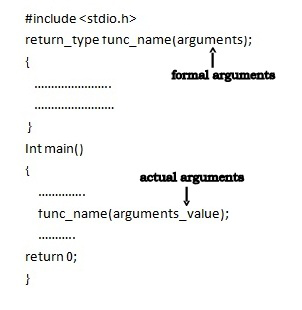
\includegraphics[width=0.5\linewidth]{P3/img/screenshot006.png}
              \caption{}
              \label{fig:parameterformalaktual}
          \end{figure}
\end{enumerate}
\subsection{Parameter Passing}
% Passing parameter merupakan aktivitas menyalurkan nilai pada 
% parameter saat memanggil fungsi. Pada umumnya, dikenal dua 
% macam passing parameter yaitu:
Parameter passing is passing a value to the parameter when calling a function.
Generally, there are two ways to pass paramaters into a function :
\begin{itemize}
    \item Pass parameter by value means to pass the
          \textbf{value} of the variable to the parameter of a function.
          % \item Pass parameter by value, yaitu menyalurkan 
          % \textbf{nilai} dari tiap parameter yang diberikan.

    \item Pass parameter by reference means to pass the
          reference of a variable \textbf{(its memory address)} to
          the paramater a function.
          % \item Pass parameter by reference, yaitu menyalurkan 
          % \textbf{alamat} dari tiap parameter yang diberikan.
\end{itemize}

\subsubsection{Passing Parameter by Value}

\begin{lstlisting}[language=c,caption = Passing by Value,label=lst:passbyvalue01]
    #include <stdio.h>

    int swapAndReturnSum(int x, int y) {
        int z;
        z = x;
        x = y;
        y = z;
        return x + y;
    }
    
    int main() {
        int a = 1;
        int b = 2;
        int sum = swapAndReturnSum(a, b);
        printf("Sum: %d\n", sum);
        printf("Value a and b now:\n");
        printf("a: %d\n", a);
        printf("b: %d\n", b);
        return 0;
    }
\end{lstlisting}

% Perhatikan potongan kode pada Listing \ref{lst:passbyvalue01}. 
% Baris 3-6 dari kode tersebut adalah operasi untuk menukar 
% nilai dari 2 variabel. Namun, apabila program tersebut 
% dijalankan, maka akan muncul output
Pay attention at the snippet above, line 3-6 of the code
in Listing \ref{lst:passbyvalue01} is a set of assignments
to swap the values of 2 variables. However, when the program
is executed, the output would be the following.
\begin{verbatim}
    sum: 3
    values a and b now:
    a: 1
    b: 2
\end{verbatim}
As you can see, the values of a and b did not swap.
When passing parameter by value, anything that is done
within the function body will have no effect on the
parameter that is "passed on" the function. The value of
the \textbf{actual parameter} will be assigned to the \textbf{formal parameter},
so we are not doing operation directly on the actual parameter.

% Nilai dari a dan b tidak bertukar. Untuk passing parameter 
% by value, apapun yang dilakukan pada function body tidak 
% akan berpengaruh pada parameter yang "dipassingkan". Nilai 
% dari parameter aktual akan diassign pada parameter formal.

\subsubsection{Passing Parameter by Reference}
% Perhatikan baris 2 pada potongan kode berikut:
Look at second line of the following code.
\begin{lstlisting}[language=c,caption = Passing by Reference,label=lst:passbyreference01]
    #include <stdio.h>

    void swap(int *x, int *y) {
        int z;
        z = *x;
        *x = *y;
        *y = z;
    }
    
    int main() {
        int a = 1;
        int b = 2;
        
        printf("Before swapping:\n");
        printf("a: %d\n", a);
        printf("b: %d\n", b);
        
        swap(&a, &b);
        
        printf("After swapping:\n");
        printf("a: %d\n", a);
        printf("b: %d\n", b);
        
        return 0;
    }
\end{lstlisting}
% Apabila program tersebut dijalankan, maka akan muncul output
The following is the ouput of the program's execution.
\begin{verbatim}
    Before swapping:
    a: 1
    b: 2
    After swapping:
    a: 2
    b: 1
\end{verbatim}

% Ketika fungsi \verb|swapAndReturnTheSum(a,b)| dipanggil, 
% alamat memori variabel a dan b "dipassingkan" pada fungsinya. 
% Sehingga pada pada potongan kode di baris 4-6, x dan y akan 
% mengacu pada memori parameter aktual yang dimasukkan di 
% baris ke 13. Ketika melakukan passing by reference, kita 
% tidak bisa memanggil fungsi dengan parameter yang tidak 
% memiliki alamat memori. Sebagai contoh 
% \verb|tukarDanKembalikansumnya(1,2)| tidak bisa dilakukan 
% karena angka 1 dan 2 bukan variabel dan tidak memiliki 
% alamat memori.
When \verb|swap(a,b)| is called,
the memory address of \verb|a| and \verb|b| is passed into
the function. Therefore, in line 4-7, the \verb|x| and
\verb|y| will point to the memory of the \textbf{actual parameter}
that is inserted in line 18, therefore we are doing assignments
directly to the actual parameter. When passing by reference,
we can't call the function with parameter that has no memory
address. As an example \verb|swapAndReturnTheSum(1,2)| cannot be
done as the number 1 and 2 doesn't have memory address.

% \subsection{Tugas Pendahuluan}
\subsection{Pre-lab Assignment}
\begin{enumerate}
    \item What is the advantages and disadvantages of function?
    \item Create a function with 2 arguments a and b of integer type that returns $a^2 + b^2$.
          % \item Masalah-masalah apa yang akan lebih mudah 
          % diselesaikan dengan menggunakan fungsi?
    \item What are the problems that can be more easily solved with functions?
\end{enumerate}

% \section{Rekursi}
\section{Recursion}
% Rekursi merujuk kepada definisi suatu hal yang dilakukan secara berulang-ulang.
Recursion refers to something that is done repeatedly
% Rekursi adalah ketika suatu fungsi dalam function bodynya memanggil fungsi itu sendiri.
Recursion in programming is when a function calls itself within its function body.
% Sebagai contoh, perhatikan potongan kode berikut:
As an example, take a look at the code below.
% \begin{lstlisting}[language=c,caption = Factorial dengan rekursi,label=lst:recursionexample01]
% int factorial(int n) 
\begin{lstlisting}[language=c,caption = Factorial with a recursion,label=lst:recursionexample01]
    int factorial(int n) {
    if (n==1)
        return 1;
    return n*factorial(n-1);
}
\end{lstlisting}
The factorial function calls another factorial function in line 4.
%Dapat dilihat bahwa fungsi factorial pada function bodynya memanggil factorial pada baris 4.
Initialy, the function $factorial(n)$ is called. This function however will return
%Pada awalnya jika fungsi $factorial(n)$ dipanggil maka dia akan mencoba untuk mengembalikan
$n\times factorial(n-1)$, then $factorial(n-1)$ will return $(n-1)\times factorial(n-1-1)$.
% $n\times factorial(n-1)$, kemudian $factorial(n-1)$ akan mengembalikan $(n-1)\times factorial(n-1-1)$.
Eventually it became like this:
% Akhirnya menjadi seperti ini:
\begin{equation*}
    \begin{split}
        factorial(n)& = n \times factorial(n-1)\\
        & = n \times (n-1) \times factorial(n-2)\\
        & = n \times (n-1) \times (n-2) \times \cdots \times 2 \times factorial(1)\\
        & = n \times (n-1) \times (n-2) \times \cdots \times 2 \times 1\\
    \end{split}
\end{equation*}

\subsection{Pre-lab Assignment}
\begin{enumerate}
    \item What are the problems that can be more easily solved with recursion?
    \item what happens if we delete the 2nd and 3rd rows in Listing \ref{lst:recursionexample01}?
    % \item Diberikan sebuah baris bilangan 1, 5, 14, 30, ... dst. Buatlah sebuah program yang mengimplementasikan fungsi rekursif untuk menentukan bilangan ke-n dari pola tersebut.
    \item Given a sequence of numbers 1, 5, 14, 30, 55, 91, ... etc. Create a program that implements a recursive function to determine the nth number in the pattern.
\end{enumerate}